\documentclass{article}
\usepackage{graphicx}
\usepackage{enumerate}
\usepackage{comment}
\usepackage[a4paper]{geometry}
\geometry{textwidth=\paperwidth, textheight=\paperheight, noheadfoot, nomarginpar}
\setlength{\topskip}{0mm}
\setlength{\parindent}{0mm}

\begin{document}
    \hrule
    \begin{center}
        \textbf{ Lamma    Tommaso    0000881007        Turno    IV }
    \end{center}
    \hrule
    \begin{center}
        {\huge Misura della caratteristica di due diodi a giunzione p-n}\\
    \end{center}
    \vspace{0.2cm}
    Lo scopo della prova era la misura della caratteristica di un diodo al Silicio ed uno al Germanio\\
    per ricavare il parametro $\eta V_T$ della legge di Schotky.\\
    Il circuito utilizzato per la prova \'e il seguente \\
    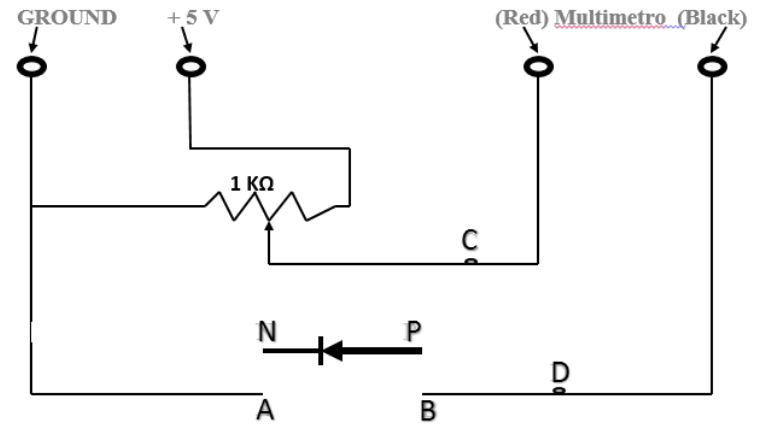
\includegraphics[width = 6cm, height = 4cm]{circuito.png}.\\
    Gli strumenti utilizzati nella prova sono:
    \begin{enumerate}[(i)]
        \item Potenziometro da 1$k\Omega$
        \item Diodi a giunzione p-n: AAZ15/OA47 Germanio, 1N914A/1N4446/1N4148 Silicio
        \item Breadboard generica
        \item Oscilloscopio ISR 622 ISO-TECH
        \item Multimetro digitale FLUKE 75
        \item Generatore di tensione continua IPS 3303 ISO-TECH
    \end{enumerate}
    I dati misurati per la calibrazione di multimetro ed oscilloscopio sono:\\
    \begin{tabular}{|p{1cm}|p{1cm}|p{1cm}|p{1cm}|}
        \hline
        $V_{mul}$ & $\delta V_{mul}$ & $V_{osc}$ & $\delta V_{osc}$ \\
        \hline
        0.099 & 0.0003 & 0.1 & 0.002\\
        0.151 & 0.0004 & 0.15 & 0.005\\
        0.199 & 0.0005 & 0.2 & 0.005\\
        0.294 & 0.0006 & 0.3 & 0.01\\
        0.394 & 0.0008 & 0.4 & 0.01\\
        0.491 & 0.0009 & 0.5 & 0.01\\
        0.591 & 0.001 & 0.6 & 0.01\\
        0.691 & 0.003 & 0.7 & 0.02\\
        0.791 & 0.003 & 0.8 & 0.02\\
        \hline
    \end{tabular}\\
    Il cui grafico in scala lineare :\\
    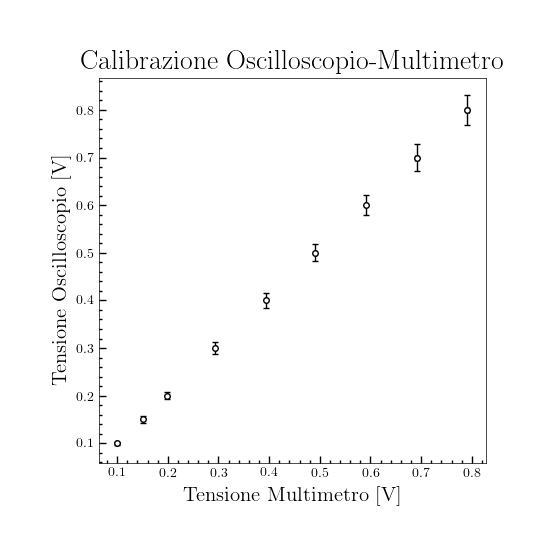
\includegraphics[width = 8cm, height = 8cm]{calibrazione/calibrazione.png}
    \newpage
    I dati misurati per il diodo al Silicio e al Germanio sono rispettivamente:\\
    \begin{tabular}{|p{1cm}|p{1cm}|p{1cm}|p{1cm}|}
        \hline
        \textbf V & $\delta$V & I & $\delta$I \\
        \hline
        0.07 & 0.01 & 0.01 & 0.0004\\
        0.08 & 0.01 & 0.01 & 0.0004\\
        0.1  & 0.01 & 0.02 & 0.0005\\
        0.12 & 0.01 & 0.04 & 0.0007\\
        0.14 & 0.01 & 0.07 & 0.001\\
        0.16 & 0.01 & 0.10 & 0.004\\
        0.18 & 0.01 & 0.16 & 0.005\\
        0.20 & 0.01 & 0.24 & 0.005\\
        0.24 & 0.01 & 0.53 & 0.008\\
        0.26 & 0.01 & 0.73 & 0.01\\
        0.28 & 0.01 & 1.07 & 0.04\\
        0.29 & 0.01 & 1.26 & 0.04\\
        0.30 & 0.01 & 1.48 & 0.04\\
        0.31 & 0.01 & 1.74 & 0.05\\
        0.32 & 0.01 & 2.03 & 0.05\\
        \hline      
    \end{tabular}
    \hspace{2cm}
    \begin{tabular}{|p{1cm}|p{1cm}|p{1cm}|p{1cm}|}
        \hline
        \textbf V & $\delta$V & I & $\delta$I \\
        \hline
        0.4 & 0.01 & 0.01 & 0.0004\\
        0.5 & 0.01 & 0.06 & 0.0009\\
        0.54 & 0.01 & 0.12 & 0.003\\
        0.56 & 0.01 & 0.2 & 0.005\\
        0.58 & 0.01 & 0.25 & 0.006\\
        0.59 & 0.01 & 0.33 & 0.006\\
        0.6 & 0.01 & 0.42 & 0.007\\
        0.61 & 0.01 & 0.5 & 0.008\\
        0.62 & 0.01 & 0.6 & 0.009\\
        0.64 & 0.01 & 0.92 & 0.01\\
        0.65 & 0.01 & 1.06 & 0.03\\
        0.66 & 0.01 & 1.27 & 0.03\\
        0.67 & 0.01 & 1.55 & 0.05\\
        0.68 & 0.01 & 1.88 & 0.05\\
        0.7 & 0.01 & 2.65 & 0.06\\
        \hline
    \end{tabular}\\
    Seguono i loro rispettivi grafici in scala semilogaritmica:\\
    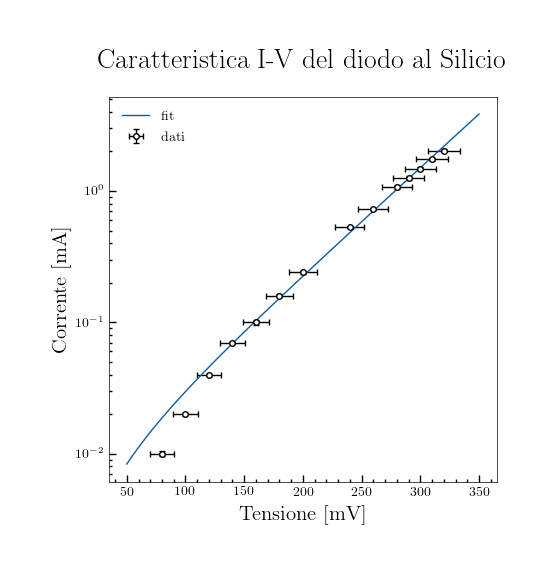
\includegraphics[width = 8cm, height = 8cm]{silicio/grafico_silicio.png}
    \hspace{2cm}
    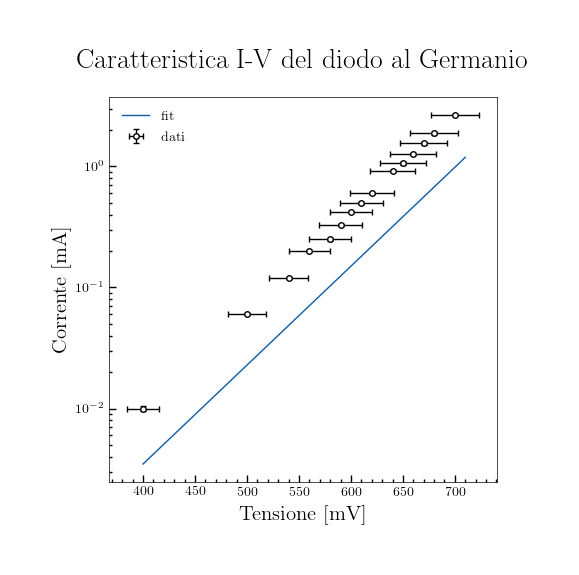
\includegraphics[width = 8cm, height = 8cm]{germanio/grafico_germanio.png}
\end{document}